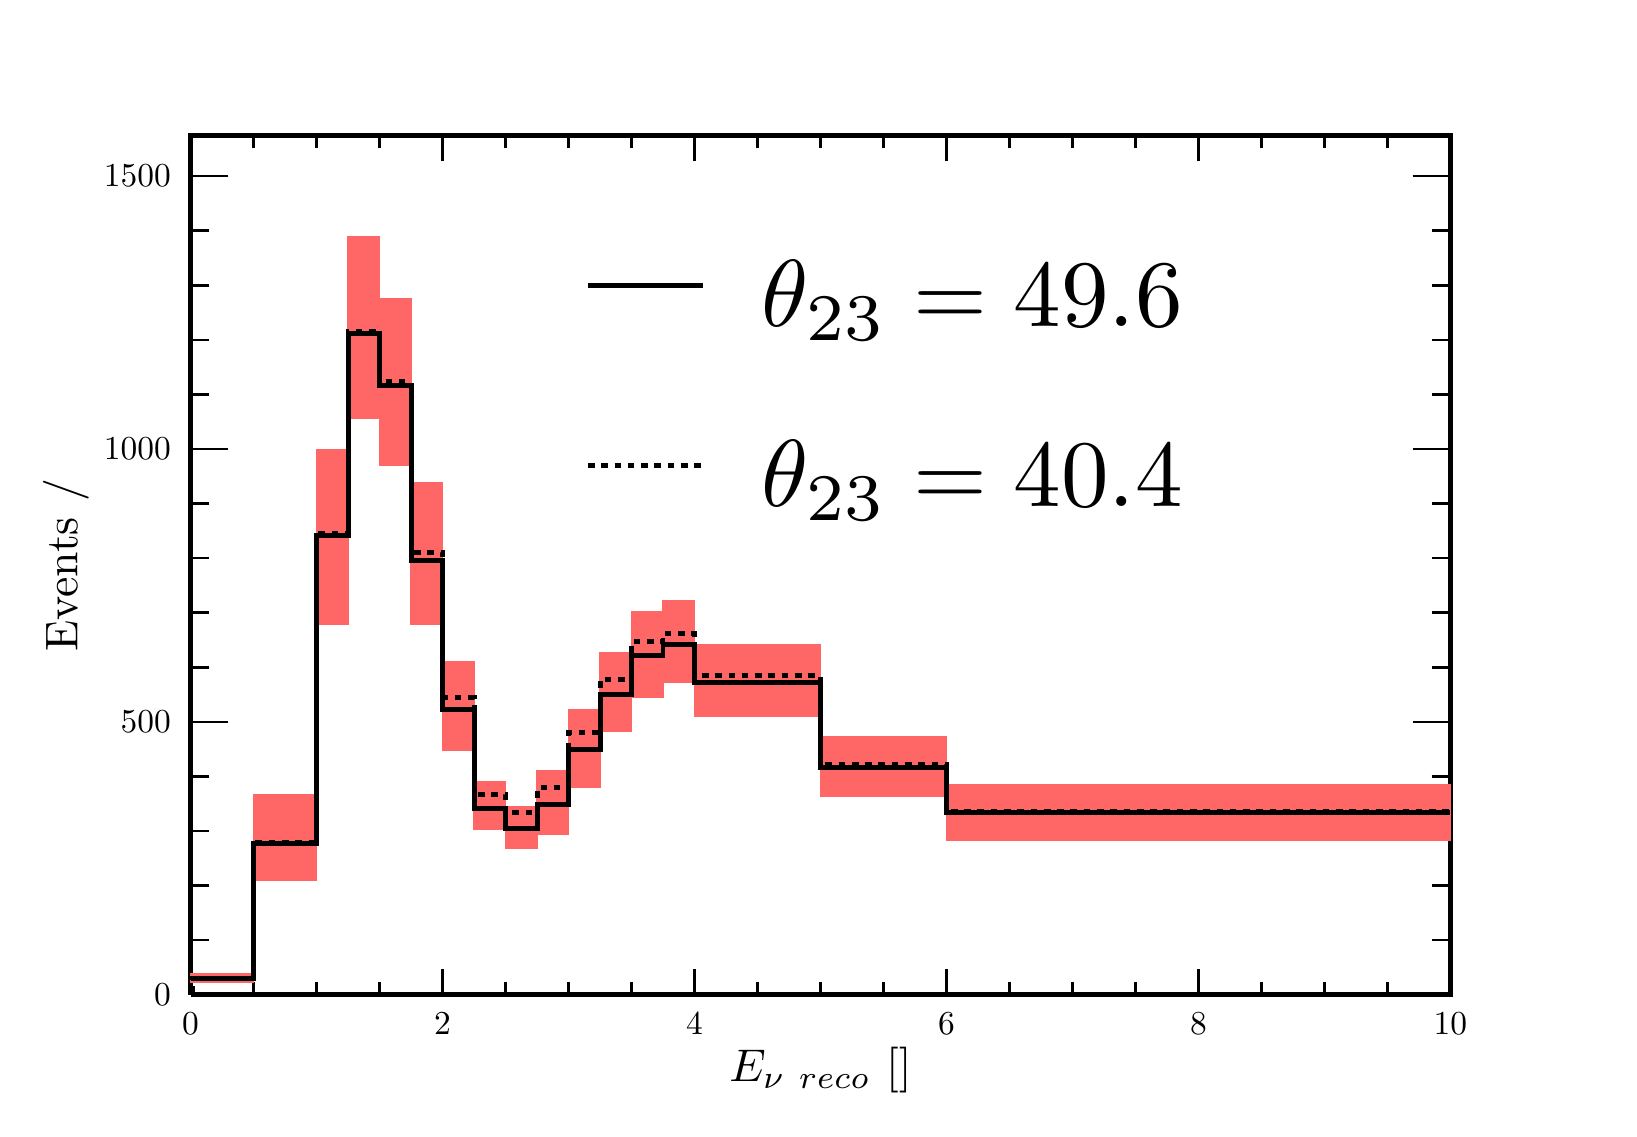
\begin{tikzpicture}
\pgfdeclareplotmark{cross} {
\pgfpathmoveto{\pgfpoint{-0.3\pgfplotmarksize}{\pgfplotmarksize}}
\pgfpathlineto{\pgfpoint{+0.3\pgfplotmarksize}{\pgfplotmarksize}}
\pgfpathlineto{\pgfpoint{+0.3\pgfplotmarksize}{0.3\pgfplotmarksize}}
\pgfpathlineto{\pgfpoint{+1\pgfplotmarksize}{0.3\pgfplotmarksize}}
\pgfpathlineto{\pgfpoint{+1\pgfplotmarksize}{-0.3\pgfplotmarksize}}
\pgfpathlineto{\pgfpoint{+0.3\pgfplotmarksize}{-0.3\pgfplotmarksize}}
\pgfpathlineto{\pgfpoint{+0.3\pgfplotmarksize}{-1.\pgfplotmarksize}}
\pgfpathlineto{\pgfpoint{-0.3\pgfplotmarksize}{-1.\pgfplotmarksize}}
\pgfpathlineto{\pgfpoint{-0.3\pgfplotmarksize}{-0.3\pgfplotmarksize}}
\pgfpathlineto{\pgfpoint{-1.\pgfplotmarksize}{-0.3\pgfplotmarksize}}
\pgfpathlineto{\pgfpoint{-1.\pgfplotmarksize}{0.3\pgfplotmarksize}}
\pgfpathlineto{\pgfpoint{-0.3\pgfplotmarksize}{0.3\pgfplotmarksize}}
\pgfpathclose
\pgfusepathqstroke
}
\pgfdeclareplotmark{cross*} {
\pgfpathmoveto{\pgfpoint{-0.3\pgfplotmarksize}{\pgfplotmarksize}}
\pgfpathlineto{\pgfpoint{+0.3\pgfplotmarksize}{\pgfplotmarksize}}
\pgfpathlineto{\pgfpoint{+0.3\pgfplotmarksize}{0.3\pgfplotmarksize}}
\pgfpathlineto{\pgfpoint{+1\pgfplotmarksize}{0.3\pgfplotmarksize}}
\pgfpathlineto{\pgfpoint{+1\pgfplotmarksize}{-0.3\pgfplotmarksize}}
\pgfpathlineto{\pgfpoint{+0.3\pgfplotmarksize}{-0.3\pgfplotmarksize}}
\pgfpathlineto{\pgfpoint{+0.3\pgfplotmarksize}{-1.\pgfplotmarksize}}
\pgfpathlineto{\pgfpoint{-0.3\pgfplotmarksize}{-1.\pgfplotmarksize}}
\pgfpathlineto{\pgfpoint{-0.3\pgfplotmarksize}{-0.3\pgfplotmarksize}}
\pgfpathlineto{\pgfpoint{-1.\pgfplotmarksize}{-0.3\pgfplotmarksize}}
\pgfpathlineto{\pgfpoint{-1.\pgfplotmarksize}{0.3\pgfplotmarksize}}
\pgfpathlineto{\pgfpoint{-0.3\pgfplotmarksize}{0.3\pgfplotmarksize}}
\pgfpathclose
\pgfusepathqfillstroke
}
\pgfdeclareplotmark{newstar} {
\pgfpathmoveto{\pgfqpoint{0pt}{\pgfplotmarksize}}
\pgfpathlineto{\pgfqpointpolar{44}{0.5\pgfplotmarksize}}
\pgfpathlineto{\pgfqpointpolar{18}{\pgfplotmarksize}}
\pgfpathlineto{\pgfqpointpolar{-20}{0.5\pgfplotmarksize}}
\pgfpathlineto{\pgfqpointpolar{-54}{\pgfplotmarksize}}
\pgfpathlineto{\pgfqpointpolar{-90}{0.5\pgfplotmarksize}}
\pgfpathlineto{\pgfqpointpolar{234}{\pgfplotmarksize}}
\pgfpathlineto{\pgfqpointpolar{198}{0.5\pgfplotmarksize}}
\pgfpathlineto{\pgfqpointpolar{162}{\pgfplotmarksize}}
\pgfpathlineto{\pgfqpointpolar{134}{0.5\pgfplotmarksize}}
\pgfpathclose
\pgfusepathqstroke
}
\pgfdeclareplotmark{newstar*} {
\pgfpathmoveto{\pgfqpoint{0pt}{\pgfplotmarksize}}
\pgfpathlineto{\pgfqpointpolar{44}{0.5\pgfplotmarksize}}
\pgfpathlineto{\pgfqpointpolar{18}{\pgfplotmarksize}}
\pgfpathlineto{\pgfqpointpolar{-20}{0.5\pgfplotmarksize}}
\pgfpathlineto{\pgfqpointpolar{-54}{\pgfplotmarksize}}
\pgfpathlineto{\pgfqpointpolar{-90}{0.5\pgfplotmarksize}}
\pgfpathlineto{\pgfqpointpolar{234}{\pgfplotmarksize}}
\pgfpathlineto{\pgfqpointpolar{198}{0.5\pgfplotmarksize}}
\pgfpathlineto{\pgfqpointpolar{162}{\pgfplotmarksize}}
\pgfpathlineto{\pgfqpointpolar{134}{0.5\pgfplotmarksize}}
\pgfpathclose
\pgfusepathqfillstroke
}
\definecolor{c}{rgb}{0.999,0.999,0.999};
\draw [color=c, fill=c] (0,0) rectangle (20,13.639);
\draw [color=c, fill=c] (2,1.3639) rectangle (18,12.2751);
\definecolor{c}{rgb}{0,0,0};
\draw [c,line width=1.8] (2,1.3639) -- (2,12.2751) -- (18,12.2751) -- (18,1.3639) -- (2,1.3639);
\definecolor{c}{rgb}{0.999,0.999,0.999};
\draw [color=c, fill=c] (2,1.3639) rectangle (18,12.2751);
\definecolor{c}{rgb}{0,0,0};
\draw [c,line width=1.8] (2,1.3639) -- (2,12.2751) -- (18,12.2751) -- (18,1.3639) -- (2,1.3639);
\draw [c,line width=1.8] (2,1.57169) -- (2.8,1.57169) -- (2.8,3.28175) -- (3.6,3.28175) -- (3.6,7.19234) -- (4,7.19234) -- (4,9.75711) -- (4.4,9.75711) -- (4.4,9.09746) -- (4.8,9.09746) -- (4.8,6.88525) -- (5.2,6.88525) -- (5.2,4.99266) --
 (5.6,4.99266) -- (5.6,3.73479) -- (6,3.73479) -- (6,3.47247) -- (6.4,3.47247) -- (6.4,3.78133) -- (6.8,3.78133) -- (6.8,4.48314) -- (7.2,4.48314) -- (7.2,5.17879) -- (7.6,5.17879) -- (7.6,5.67814) -- (8,5.67814) -- (8,5.81819) -- (8.4,5.81819) --
 (8.4,5.33518) -- (10,5.33518) -- (10,4.25465) -- (11.6,4.25465) -- (11.6,3.67823) -- (18,3.67823);
\draw [c,line width=0.9] (2,1.3639) -- (18,1.3639);
\draw [c,line width=0.9] (2,1.69123) -- (2,1.3639);
\draw [c,line width=0.9] (2.8,1.52756) -- (2.8,1.3639);
\draw [c,line width=0.9] (3.6,1.52756) -- (3.6,1.3639);
\draw [c,line width=0.9] (4.4,1.52756) -- (4.4,1.3639);
\draw [c,line width=0.9] (5.2,1.69123) -- (5.2,1.3639);
\draw [c,line width=0.9] (6,1.52756) -- (6,1.3639);
\draw [c,line width=0.9] (6.8,1.52756) -- (6.8,1.3639);
\draw [c,line width=0.9] (7.6,1.52756) -- (7.6,1.3639);
\draw [c,line width=0.9] (8.4,1.69123) -- (8.4,1.3639);
\draw [c,line width=0.9] (9.2,1.52756) -- (9.2,1.3639);
\draw [c,line width=0.9] (10,1.52756) -- (10,1.3639);
\draw [c,line width=0.9] (10.8,1.52756) -- (10.8,1.3639);
\draw [c,line width=0.9] (11.6,1.69123) -- (11.6,1.3639);
\draw [c,line width=0.9] (12.4,1.52756) -- (12.4,1.3639);
\draw [c,line width=0.9] (13.2,1.52756) -- (13.2,1.3639);
\draw [c,line width=0.9] (14,1.52756) -- (14,1.3639);
\draw [c,line width=0.9] (14.8,1.69123) -- (14.8,1.3639);
\draw [c,line width=0.9] (15.6,1.52756) -- (15.6,1.3639);
\draw [c,line width=0.9] (16.4,1.52756) -- (16.4,1.3639);
\draw [c,line width=0.9] (17.2,1.52756) -- (17.2,1.3639);
\draw [c,line width=0.9] (18,1.69123) -- (18,1.3639);
\draw [anchor=base] (2,0.859255) node[scale=1.20912, color=c, rotate=0]{0};
\draw [anchor=base] (5.2,0.859255) node[scale=1.20912, color=c, rotate=0]{2};
\draw [anchor=base] (8.4,0.859255) node[scale=1.20912, color=c, rotate=0]{4};
\draw [anchor=base] (11.6,0.859255) node[scale=1.20912, color=c, rotate=0]{6};
\draw [anchor=base] (14.8,0.859255) node[scale=1.20912, color=c, rotate=0]{8};
\draw [anchor=base] (18,0.859255) node[scale=1.20912, color=c, rotate=0]{10};
\draw (10,0.403714) node[scale=1.65459, color=c, rotate=0]{$E_{\nu~\text{reco}}$ [\si{\GeV}]};
\draw [c,line width=0.9] (2,12.2751) -- (18,12.2751);
\draw [c,line width=0.9] (2,11.9477) -- (2,12.2751);
\draw [c,line width=0.9] (2.8,12.1114) -- (2.8,12.2751);
\draw [c,line width=0.9] (3.6,12.1114) -- (3.6,12.2751);
\draw [c,line width=0.9] (4.4,12.1114) -- (4.4,12.2751);
\draw [c,line width=0.9] (5.2,11.9477) -- (5.2,12.2751);
\draw [c,line width=0.9] (6,12.1114) -- (6,12.2751);
\draw [c,line width=0.9] (6.8,12.1114) -- (6.8,12.2751);
\draw [c,line width=0.9] (7.6,12.1114) -- (7.6,12.2751);
\draw [c,line width=0.9] (8.4,11.9477) -- (8.4,12.2751);
\draw [c,line width=0.9] (9.2,12.1114) -- (9.2,12.2751);
\draw [c,line width=0.9] (10,12.1114) -- (10,12.2751);
\draw [c,line width=0.9] (10.8,12.1114) -- (10.8,12.2751);
\draw [c,line width=0.9] (11.6,11.9477) -- (11.6,12.2751);
\draw [c,line width=0.9] (12.4,12.1114) -- (12.4,12.2751);
\draw [c,line width=0.9] (13.2,12.1114) -- (13.2,12.2751);
\draw [c,line width=0.9] (14,12.1114) -- (14,12.2751);
\draw [c,line width=0.9] (14.8,11.9477) -- (14.8,12.2751);
\draw [c,line width=0.9] (15.6,12.1114) -- (15.6,12.2751);
\draw [c,line width=0.9] (16.4,12.1114) -- (16.4,12.2751);
\draw [c,line width=0.9] (17.2,12.1114) -- (17.2,12.2751);
\draw [c,line width=0.9] (18,11.9477) -- (18,12.2751);
\draw [c,line width=0.9] (2,1.3639) -- (2,12.2751);
\draw [c,line width=0.9] (2.48,1.3639) -- (2,1.3639);
\draw [c,line width=0.9] (2.24,2.05703) -- (2,2.05703);
\draw [c,line width=0.9] (2.24,2.75017) -- (2,2.75017);
\draw [c,line width=0.9] (2.24,3.4433) -- (2,3.4433);
\draw [c,line width=0.9] (2.24,4.13643) -- (2,4.13643);
\draw [c,line width=0.9] (2.48,4.82957) -- (2,4.82957);
\draw [c,line width=0.9] (2.24,5.5227) -- (2,5.5227);
\draw [c,line width=0.9] (2.24,6.21584) -- (2,6.21584);
\draw [c,line width=0.9] (2.24,6.90897) -- (2,6.90897);
\draw [c,line width=0.9] (2.24,7.60211) -- (2,7.60211);
\draw [c,line width=0.9] (2.48,8.29524) -- (2,8.29524);
\draw [c,line width=0.9] (2.24,8.98838) -- (2,8.98838);
\draw [c,line width=0.9] (2.24,9.68151) -- (2,9.68151);
\draw [c,line width=0.9] (2.24,10.3746) -- (2,10.3746);
\draw [c,line width=0.9] (2.24,11.0678) -- (2,11.0678);
\draw [c,line width=0.9] (2.48,11.7609) -- (2,11.7609);
\draw [c,line width=0.9] (2.48,11.7609) -- (2,11.7609);
\draw [anchor= east] (1.9,1.3639) node[scale=1.20912, color=c, rotate=0]{0};
\draw [anchor= east] (1.9,4.82957) node[scale=1.20912, color=c, rotate=0]{500};
\draw [anchor= east] (1.9,8.29524) node[scale=1.20912, color=c, rotate=0]{1000};
\draw [anchor= east] (1.9,11.7609) node[scale=1.20912, color=c, rotate=0]{1500};
\draw (0.416,6.81948) node[scale=1.65459, color=c, rotate=90]{Events / \si{\GeV}};
\draw [c,line width=0.9] (18,1.3639) -- (18,12.2751);
\draw [c,line width=0.9] (17.52,1.3639) -- (18,1.3639);
\draw [c,line width=0.9] (17.76,2.05703) -- (18,2.05703);
\draw [c,line width=0.9] (17.76,2.75017) -- (18,2.75017);
\draw [c,line width=0.9] (17.76,3.4433) -- (18,3.4433);
\draw [c,line width=0.9] (17.76,4.13643) -- (18,4.13643);
\draw [c,line width=0.9] (17.52,4.82957) -- (18,4.82957);
\draw [c,line width=0.9] (17.76,5.5227) -- (18,5.5227);
\draw [c,line width=0.9] (17.76,6.21584) -- (18,6.21584);
\draw [c,line width=0.9] (17.76,6.90897) -- (18,6.90897);
\draw [c,line width=0.9] (17.76,7.60211) -- (18,7.60211);
\draw [c,line width=0.9] (17.52,8.29524) -- (18,8.29524);
\draw [c,line width=0.9] (17.76,8.98838) -- (18,8.98838);
\draw [c,line width=0.9] (17.76,9.68151) -- (18,9.68151);
\draw [c,line width=0.9] (17.76,10.3746) -- (18,10.3746);
\draw [c,line width=0.9] (17.76,11.0678) -- (18,11.0678);
\draw [c,line width=0.9] (17.52,11.7609) -- (18,11.7609);
\draw [c,line width=0.9] (17.52,11.7609) -- (18,11.7609);
\definecolor{c}{rgb}{1,0.4,0.4};
\draw [color=c, fill=c] (2,1.52109) rectangle (2.8,1.63215);
\draw [color=c, fill=c] (2.8,2.80955) rectangle (3.6,3.90192);
\draw [color=c, fill=c] (3.6,6.06063) rectangle (4,8.2942);
\draw [color=c, fill=c] (4,8.6774) rectangle (4.4,10.9896);
\draw [color=c, fill=c] (4.4,8.08761) rectangle (4.8,10.2035);
\draw [color=c, fill=c] (4.8,6.06386) rectangle (5.2,7.86839);
\draw [color=c, fill=c] (5.2,4.46483) rectangle (5.6,5.58935);
\draw [color=c, fill=c] (5.6,3.46701) rectangle (6,4.06584);
\draw [color=c, fill=c] (6,3.22618) rectangle (6.4,3.75564);
\draw [color=c, fill=c] (6.4,3.39796) rectangle (6.8,4.21271);
\draw [color=c, fill=c] (6.8,4.0014) rectangle (7.2,4.99216);
\draw [color=c, fill=c] (7.2,4.70191) rectangle (7.6,5.70682);
\draw [color=c, fill=c] (7.6,5.1371) rectangle (8,6.22456);
\draw [color=c, fill=c] (8,5.33476) rectangle (8.4,6.369);
\draw [color=c, fill=c] (8.4,4.89629) rectangle (10,5.81331);
\draw [color=c, fill=c] (10,3.88193) rectangle (11.6,4.6433);
\draw [color=c, fill=c] (11.6,3.32745) rectangle (18,4.03945);
\definecolor{c}{rgb}{0,0,0};
\draw [c,line width=1.8] (2,1.57169) -- (2.8,1.57169) -- (2.8,3.28175) -- (3.6,3.28175) -- (3.6,7.19234) -- (4,7.19234) -- (4,9.75711) -- (4.4,9.75711) -- (4.4,9.09746) -- (4.8,9.09746) -- (4.8,6.88525) -- (5.2,6.88525) -- (5.2,4.99266) --
 (5.6,4.99266) -- (5.6,3.73479) -- (6,3.73479) -- (6,3.47247) -- (6.4,3.47247) -- (6.4,3.78133) -- (6.8,3.78133) -- (6.8,4.48314) -- (7.2,4.48314) -- (7.2,5.17879) -- (7.6,5.17879) -- (7.6,5.67814) -- (8,5.67814) -- (8,5.81819) -- (8.4,5.81819) --
 (8.4,5.33518) -- (10,5.33518) -- (10,4.25465) -- (11.6,4.25465) -- (11.6,3.67823) -- (18,3.67823);
\draw [c,dash pattern=on 2.40pt off 2.40pt ,line width=1.8] (2.02865,1.39255) -- (2.02865,1.56994) -- (2.8,1.56994) -- (2.8,3.29586) -- (3.6,3.29586) -- (3.6,7.2227) -- (4,7.2227) -- (4,9.78207) -- (4.4,9.78207) -- (4.4,9.14752) -- (4.8,9.14752) --
 (4.8,6.97999) -- (5.2,6.97999) -- (5.2,5.13514) -- (5.6,5.13514) -- (5.6,3.91218) -- (6,3.91218) -- (6,3.67435) -- (6.4,3.67435) -- (6.4,3.99324) -- (6.8,3.99324) -- (6.8,4.68989) -- (7.2,4.68989) -- (7.2,5.37035) -- (7.6,5.37035) -- (7.6,5.8458) --
 (8,5.8458) -- (8,5.95778) -- (8.4,5.95778) -- (8.4,5.41806) -- (10,5.41806) -- (10,4.28524) -- (11.6,4.28524) -- (11.6,3.68695) -- (18,3.68695);
\definecolor{c}{rgb}{1,1,1};
\draw [color=c, fill=c] (6.73352,6.9341) rectangle (15.1003,11.5186);
\definecolor{c}{rgb}{0,0,0};
\draw [anchor=base west] (8.82522,9.85673) node[scale=3.43646, color=c, rotate=0]{$\theta_{23} = \ang{49.6}$};
\draw [c,line width=1.8] (7.04728,10.3725) -- (8.51146,10.3725);
\draw [anchor=base west] (8.82522,7.56447) node[scale=3.43646, color=c, rotate=0]{$\theta_{23} = \ang{40.4}$};
\draw [c,dash pattern=on 2.40pt off 2.40pt ,line width=1.8] (7.04728,8.08023) -- (8.51146,8.08023);
\end{tikzpicture}
